\documentclass[twocolumn, 12pt]{article}    % two-column because cheat sheets fit like that
\usepackage[utf8]{inputenc}
\usepackage{amsmath}    % allows math to happen
\usepackage{marvosym}
\usepackage{textcomp}
\usepackage{geometry}   % allows you to change the margins and headers/footers, and more
\usepackage{array}
\usepackage{wrapfig}
\usepackage{multirow} 
\usepackage{graphicx}   % allows for inclusion of graphics or several types, i think
\usepackage{float}      % SUPER  IMPORTANT. lets you tell LaTeX where to put your graphics, as opposed to where it feels
\usepackage{wrapfig}    % Lets text wrap around figures, more relevant for reports really
\usepackage{caption}
\usepackage{amssymb}    
\usepackage{ulem}       % allows strikethrough and some
\usepackage[table]{xcolor}  % enhances tables by allowing colors to happen. notably, as background/fill colors
\usepackage{bondgraph}  % allows bond graphs
\usepackage{caption}    % lots of control of captions and caption geometries
\usepackage{comment} % allows block comments to occur
\usepackage{ragged2e}

\geometry{margin=.5in}      % this allows for a lot to fit on the page

\begin{document}
\RaggedRight
\footnotesize                      % small because, it's a cheat sheet after all, why not cram it


\section*{Design of Experiments}
\subsubsection*{Levi Barker \hspace{55pt} U0959362}
\underline{Variables}
\begin{itemize}
    \item Numerical
    \begin{itemize}
        \item Continuous
        \item Discrete - known interval
    \end{itemize}
    \item Categorical
    \begin{itemize}
        \item Regular categorical
        \item Ordinal - interval not implied
        \item Dichotomous - binary, Bernoulli
    \end{itemize}
    \item Role
    \begin{itemize}
        \item Explanatory - the factor(s) changed
        \item Response - response to explanatory  
    \end{itemize}
    \item Misc.
    \begin{itemize}
        \item Factors - condition imposed
        \item Treatment/Level - the magnitude of the factor (concentration, etc)
    \end{itemize}
\end{itemize}

\underline{Terminology}
\begin{itemize}
    \item Skew left - mean\(<\)med. Skew right - mean\(>\)med
    \item Kurtosis - deviation from normal due to tail thickness
    \item Error types
\end{itemize}


\begin{figure}[h!]
    \centering
    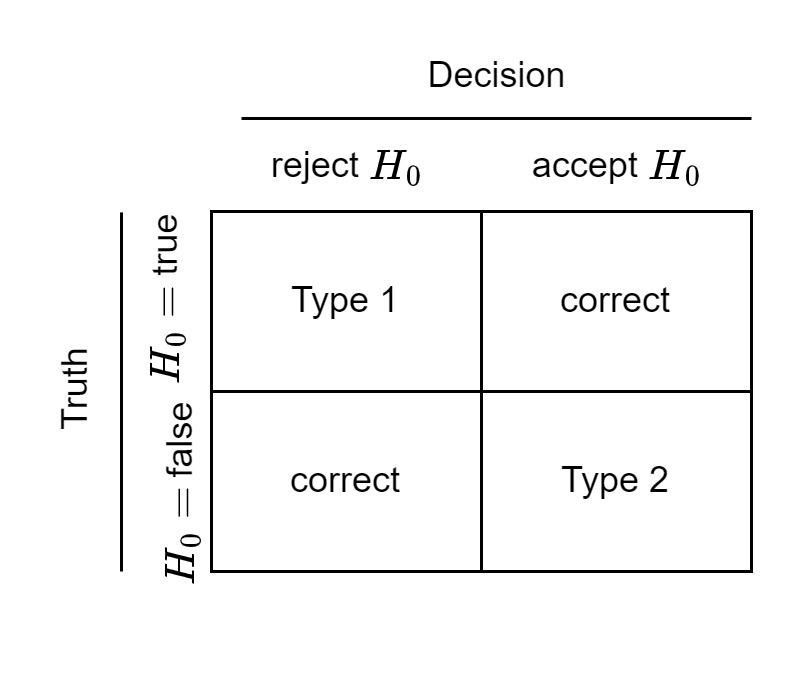
\includegraphics[width=0.35\textwidth]{ErrorTypes.jpg}
\end{figure}


\subsection*{t-test}
Standard deviation is variance\(^2\)
If n is big, or Greek letters, or population parameters, use Z-test. Otherwise:

\begin{equation*}
    \text{Single Group Mean} \hspace{30pt} t = \frac{\Bar{x}-(null)}{s/\sqrt{n}} \hspace{30pt} df = n-1
\end{equation*}
\begin{equation*}
    \text{Compare Two Means} \hspace{30pt} t = \frac{\Bar{x}_1-\Bar{x}_2-(null)}{\sqrt{\frac{s_1^2}{n_1} + \frac{s_2^2}{n_2}}}   
\end{equation*}
\begin{equation*}
    df_{max} = n_1+n_2-2 \hspace{30pt} df_{min} = min(n_1-1,n_2-1)
\end{equation*}
\begin{equation*}
    \text{Paired/Dependent} \hspace{30pt} t = \frac{\Bar{x}_{dif} - (null)}{s_{dif}/\sqrt{n}}  \hspace{30pt} df = n-1
\end{equation*}


\subsection*{Confidence Interval}
\begin{table}[h!]
    \footnotesize
    \centering
    \begin{tabular}{lccc}
        Lower & \(CI_L = \Bar{x}-t^*_\alpha SE\) & \((-\infty, \#)\) & \(SE = s/\sqrt{n}\) \\
        Upper & \(CI_U = \Bar{x}+t^*_\alpha SE\) & \((\#, \infty)\) & \(SE = s/\sqrt{n}\) \\
        Two-Tailed & \(CI_2 = \Bar{x}\pm t^*_{\alpha/2}SE\) & \((\#, \#)\) & \(SE = s/\sqrt{n}\)
    \end{tabular}
\end{table}
If (null) is within the CI, the sample likely came from the same distribution. (Use \(t^*\) from the table, not the t calculated).


\subsection*{Hypothesis Steps}
\begin{enumerate}
    \item Set hypotheses
    \item Choose correct test statistic
    \item Check assumptions and conditions
    \item State decisions and draw picture
    \item Calculate test statistic
    \item Make decision and interpret in context with words
\end{enumerate}
p-value is the probability that what you saw happened if the null is true. If p is low, the null must go.


\subsection*{Regression}
\begin{equation*}
    \text{Estimate} \hspace{30pt} \hat{y} = b_0 + b_1x_1 + ... + b_nx_{n-1}
\end{equation*}
\begin{equation*}
    \text{Truth} \hspace{30pt} y = \beta_0 + \beta_1x_1 + ... +\beta_nx_{n-1} + \varepsilon
\end{equation*}

\begin{table}[h!]
    \centering
    \footnotesize
    \begin{tabular}{lccccc}
        Source & \(df\) & SS & MS & \(F-stat\) & \(F^*\)  \\
        \hline
        Regres. & \(df_R\) & \(SS_R\) & \(MS_R\) & \(F\)& table\\
        Error & \(df_E\) & \(SS_E\) & \(MS_E \) & \\
        Total & \(df_T\) & \(SS_T\) & \\
        \hline
    \end{tabular}
\end{table}
\begin{equation*}
    df_E=df_T-df_R \hspace{30pt} MS_R = \frac{SS_R}{df_R} \hspace{30pt} MS_E = \frac{SS_E}{df_E}
\end{equation*}
\begin{equation*}
    F =\frac{MS_R}{MS_E} \hspace{30pt} df_T = df_R+df_E \hspace{30pt} p = \text{\# predictors}
\end{equation*}
\begin{equation*}
    R = \frac{SS_R}{SS_T} \hspace{30pt} R^2_{adj} = 1- \left(\frac{SS_E}{SS_T} \right) \left( \frac{n-1}{n-p-1} \right)
\end{equation*}


\subsection*{ANOVA and Pals}
\begin{itemize}
    \item \underline{Completely Random Design (CRD)}: Entirely randomized, everywhere
    \item \underline{Fixed Effects Models}: can only be used to conclude about the exact levels used
    \item \underline{Random Effects Models}: can use to infer about entire population
    \item \(F\) = var(between groups)/var(within groups) = \(\frac{MSG}{MSE}\)
    \item Conditions:
        \begin{enumerate}
            \item Independent, random, \(N<10\%\) of pop.
            \item \(\sim\)Normal \(\longrightarrow\) residuals, Shapiro-Wilks, QQ-Plot
            \item Var across groups is roughly equal \(\longrightarrow\) Bartlett's
        \end{enumerate}
\end{itemize}
\subsubsection*{Single Factor ANOVA}
\begin{align*}
    H_0:& \mu_i=....\mu_a \hspace{30pt} &\text{or} \hspace{5pt} \tau_i =0\\
    H_A:& \mu_i \neq \mu_{i'}           &\text{for any pair of } i,i'
\end{align*}
\begin{table}[h!]
    \footnotesize
    \begin{tabular}{lcc}
        Effects Model: & \(y_{ij} = \mu + \tau_i + \varepsilon_{ij}\) & \(N=an\) \\
        Means Model: & \(y_{ij} = \mu_i + \varepsilon_{ij}\) & \(\mu_i = \mu +\tau_i\)\\
        Regression Model: &  \(\hat{y} = \mu + \sum b_ix_i\) & \(x_i = 0 \hspace{2.5pt} \text{or} \hspace{2.5pt} 1\)
    \end{tabular}
\end{table}
\subsubsection*{Factorial ANOVA}
\begin{equation*}
    y_{ij} = \mu + \hspace{-7.5pt} \underbrace{\tau_i}_{\text{A effects}} \hspace{-7.5pt} + \hspace{-7.5pt} \overbrace{\beta_j}^{\text{B effects}} \hspace{-7.5pt} + \hspace{-17.5pt} \underbrace{(\tau\beta)_{ij}}_{\text{interaction effects}} \hspace{-17.5pt} + \varepsilon_{ijk} \hspace{10pt} \begin{cases} 
        i = 1,2,...,a\\
        j = 1,2,...,b\\
        k = 1,2,...,n
    \end{cases} 
\end{equation*}
\begin{align*}
    A &\hspace{5pt}\begin{cases}
        H_0: &\tau_1=\tau_2=...=\tau_a\\
        H_A: &\text{any} \hspace{5pt} \tau_i \neq0
    \end{cases}\\
    B &\hspace{5pt} \begin{cases}
        H_0: &\beta_1 = \beta_2=...=\beta_b=0\\
        H_A: &\text{any} \hspace{5pt} \beta_i \neq 0
    \end{cases}\\
    AB &\hspace{5pt} \begin{cases}
        H_0: &(\tau \beta)_{11} = (\tau\beta)_{12} =...=(\tau\beta)_{ij}\\
        H_A: &\text{any} \hspace{5pt} (\tau\beta)_{ij} \neq 0
    \end{cases}
\end{align*}
Post-Hoc: multiple t-tests increases type-I error likelihood. Use correction or Tukey to avoid\\
\underline{Main Effects}:
\begin{equation*}
    A = \frac{1}{2} (Ab + AB - ab - aB ) = avg(\text{factor}_{\text{on}}) - avg(\text{factor}_{\text{off}})
\end{equation*}
\underline{Interaction Effects}:
\begin{equation*}
    AB = \frac{1}{2} (Ab + aB - ab - AB) = avg(\text{mixed}) - avg(\text{!mixed})
\end{equation*}


\subsection*{Blocking}
Block for uncontrollable factors (eg. height, sex, etc.) or fatigue/learning\\
\underline{Latin Squares}:
\begin{itemize}
    \item Do the sudoku, but also ensure that factor \(i\) proceeds factor \(i+1\) the same number of times it follows
    \item Blocks for two factors. Graeco-Latin Squares blocks for three factors
\end{itemize}



\subsection*{\(2^k\) Design}
\begin{itemize}
    \item Same conditions as ANOVA
    \item Each factor is high/low or present/not present
\end{itemize}
\begin{equation*}
    y_{ijkl} = \mu + \tau_i + \beta_j + \gamma_k + (\tau\beta)_{ij} + (\tau\gamma)_{ik} + (\beta\gamma)_{jk} + (\tau\beta\gamma)_{ijk} +\varepsilon_{ijkl}
\end{equation*}

\[\text{Sample } 2^2 \text{ Experimental Design} \hspace{20pt}
\begin{matrix}
        & I & A & B & AB\\
    (1) & + & - & - & +\\
    a   & + & + & - & -\\
    b   & + & - & + & -\\
    ab  & + & + & + & +
\end{matrix}\]
\begin{equation*}
    \text{effect size}_j = \frac{1}{\Gamma n }(contrast_j)  \hspace{30pt} \Gamma= 2^{k-1}
\end{equation*}
\begin{equation*}
        \text{contrast}_j = \sum_{i=\text{rows}} sgn(i,j) * \sum_i^n \text{replicates}
\end{equation*}
\begin{equation*}
    y = \text{grand mean} + \frac{1}{2} \sum \text{(effect size)}*\text{(factor)} \hspace{10pt} \text{factors} = -1,1
\end{equation*}
\subsubsection*{Fold-over Designs}
After performing a fractional factorial design, the confounding may be undesirable. A fold-over design flips the sign of one (or more) of the generators, and the same fractional factorial design is repeated (assuming 3 factor and higher interactions are non-significant).
\begin{align*}
    [i] =& \text{ effect size from standard generator}\\
    [i]' =& \text{ effect size after flipping one or more generators}
\end{align*}
\begin{equation*}
    \begin{matrix}
            \text{isolates}\\ \text{mains}
    \end{matrix} = \frac{1}{2}([i]+[i]') \hspace{30pt} \begin{matrix}
            \text{isolates} \\ \text{2-ways}
    \end{matrix} = \frac{1}{2}([i]-[i]')
\end{equation*}
\subsection*{Missing Data}
\begin{itemize}
    \item List-wise Deletion: If any element is missing, omit entire entry
    \item Pairwise Deletion: Only omit entry if relevant to test
    \item Hot-deck Imputation: Insert a random value within range of extant data
    \item Mean Substitution: Insert mean of data 
    \item Regression Substitution: Perform a regression to insert data point(s)
    \item Maximum Likelihood: Generate and try \(\geq\) 1000 values, do stats to find best entry
\end{itemize}
\subsection*{DOE Process}
\begin{figure}[h!]
    \centering
    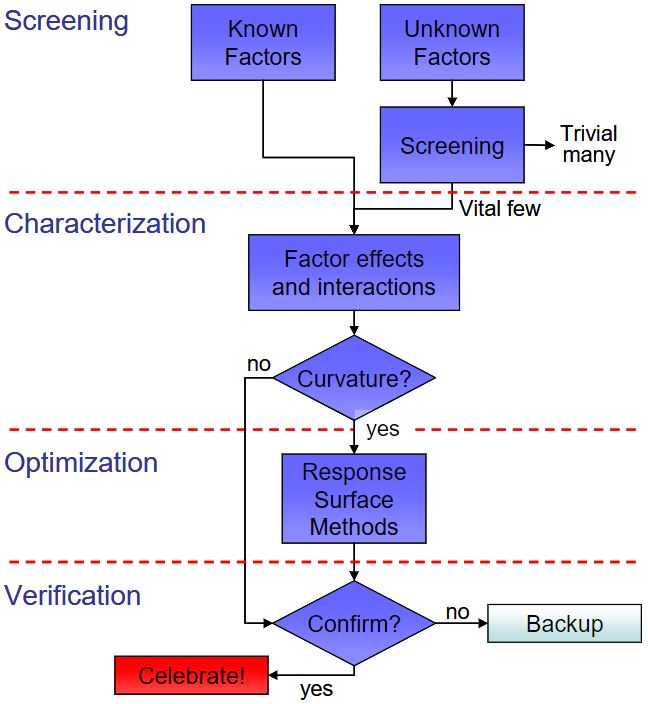
\includegraphics[width=0.4\textwidth]{DOEProcess.jpg}
\end{figure}


\end{document}